% Chapter 2 (two-cause rewrite, 2026-11). Literature only: no result of this thesis is quoted here.
% Old text: chapters_old/chapter2.tex (git tag thesis-pre-two-causes).
\chapter{Background Theory and Literature Review}
\label{ch:background}

This chapter gives the background of the thesis and reviews the related studies. In the
following, we first summarise document understanding and \gls{kie}
(Section~\ref{sec:c2-s1}) and the basics of continual learning (Section~\ref{sec:c2-s2}).
Then, we review the four lines of work that our study builds on: the shift of the background
label (Section~\ref{sec:c2-s3}), separated readouts and session identification
(Section~\ref{sec:c2-s4}), latent and compressed replay (Section~\ref{sec:c2-s5}) and
continual learning with pre-trained models (Section~\ref{sec:c2-s6}). After that, we review
continual learning for documents (Section~\ref{sec:c2-s7}). Finally, we state the research
gaps and position our work (Section~\ref{sec:c2-s8}).

% =============================================================================
\section{Document Understanding and Key-Information Extraction}
\label{sec:c2-s1}

\paragraph{The task.} Administrative documents such as forms, invoices and receipts are one
of the most widely used media to exchange information between organisations, which raises
the need for systems that read them automatically. \Gls{kie} is the task of finding the
fields of a schema in such a document, e.g., the total amount of a receipt or the answer to
a question in a form. A document is first read by an \gls{ocr} engine, which returns its
words and their bounding boxes. The dominant formulation then treats \gls{kie} as token
labelling: every token receives a tag in the \gls{bio} scheme, where B-$c$ and I-$c$ mark
the beginning and the inside of an entity of class $c$, and the tag ``O'' marks every token
that belongs to no entity. The model is trained with a token-level cross-entropy and scored
by the F1 of the extracted entities~\citep{tjong2003conll}. This formulation gives one
output format for all datasets and fits the encoder-only models that dominate the field;
hence, we adopt it in this thesis.

A document differs from a sentence in three ways that matter for our study. First, it is
spatially structured: the role of a token is often decided by its position and not by its
neighbouring words, e.g., a question and its answer in a form. Second, it is multimodal:
the text, the layout and the image jointly decide the meaning. Third, most tokens of a page
are not entities; hence, the tag ``O'' is by far the most frequent label, and how a model
treats it decides a large part of its accuracy.

\paragraph{Layout-aware encoders.} Recent studies on visually-rich documents mainly consist
of layout-aware encoders and generative models. LayoutLM~\citep{xu2020layoutlm} adds the
bounding box of every token to the input of a BERT-style
encoder~\citep{devlin2019bert}, and LayoutLMv2~\citep{xu2021layoutlmv2} adds the page
image and pre-training objectives that align the text with it.
LayoutLMv3~\citep{huang2022layoutlmv3} removes the convolutional vision backbone: the image
enters as patches, as in a vision transformer, and the model is pre-trained with masked
language modelling, masked image modelling and a word-patch alignment objective
(Figure~\ref{fig:layoutlmv3-components}). Other designs change how the modalities are
combined. For instance, LiLT~\citep{wang2022lilt} separates the layout stream from the text
stream, so that one layout model can be paired with text encoders of different languages.
As another example, BROS~\citep{hong2022bros} uses no image input and encodes the relative
positions of the text boxes, DocFormer~\citep{appalaraju2021docformer} shares the spatial
embeddings between the text and the image streams, and
GeoLayoutLM~\citep{luo2023geolayoutlm} adds geometric pre-training tasks. Generative models
such as Donut~\citep{kim2022donut} and UDOP~\citep{tang2023udop} produce the fields as a
text sequence, in the case of Donut without an \gls{ocr} engine.

\begin{figure}[!htbp]
  \centering
  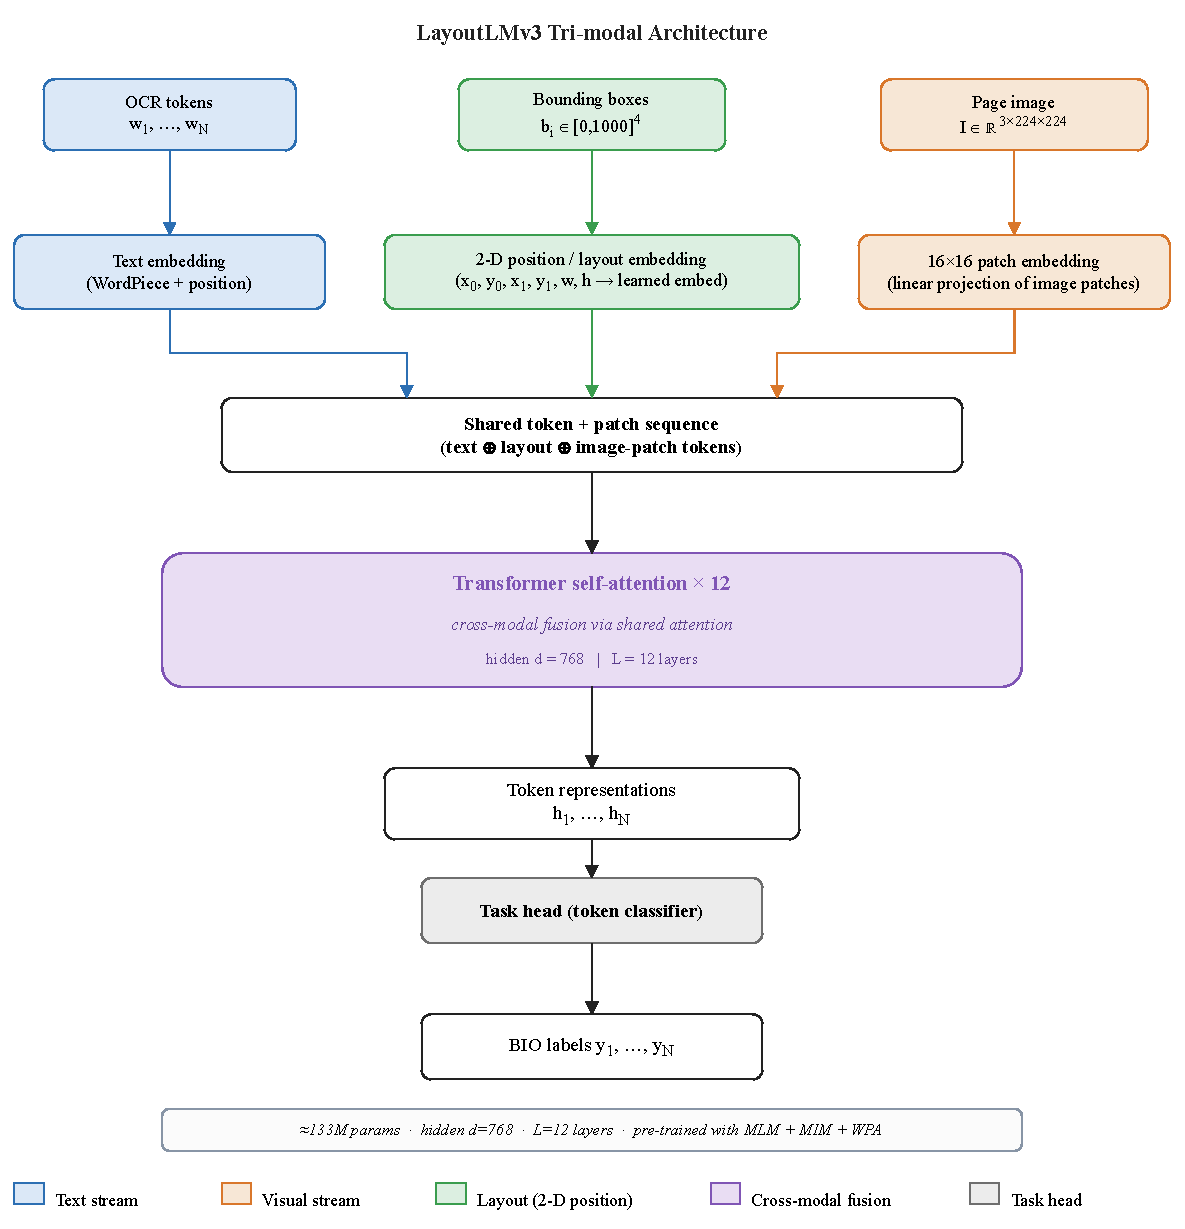
\includegraphics[width=0.72\linewidth]{layoutlmv3_components.pdf}
  \caption[The LayoutLMv3 encoder]{\textbf{The LayoutLMv3 encoder.} The \gls{ocr} tokens,
  their bounding boxes and the image patches are embedded into one sequence, which twelve
  transformer layers process jointly. A linear head maps the feature of every token to its
  \gls{bio} tag.}
  \label{fig:layoutlmv3-components}
\end{figure}

\paragraph{The fixed-label assumption.} All these models are trained once on all the data,
with a classifier sized to a fixed set of labels. However, real-world documents arrive in
sequence: a new vendor brings a new layout, a new language is added, and a new field must
be extracted that the earlier annotation did not cover. Retraining on all the data at each
change is costly, and it is not possible when the earlier documents may no longer be kept.
We use LayoutLMv3 as the main encoder of this thesis because it is the most widely adopted
encoder of this family, and LiLT, BROS and BERT to examine whether the findings depend on
the encoder (Chapter~\ref{ch:experimental-setup}).

% =============================================================================
\section{Catastrophic Forgetting and Continual Learning}
\label{sec:c2-s2}

\paragraph{Catastrophic forgetting.} Continual learning trains a model on a sequence of
sessions while it retains what it learned from the earlier ones. Its main obstacle is
catastrophic forgetting~\citep{mccloskey1989catastrophic}: when a network is trained on
new data only, the gradient steps overwrite the weights that encoded the old data, and the
old performance falls sharply. A model must therefore stay plastic enough to learn the new
session and stable enough to keep the old ones, which is known as the stability-plasticity
dilemma. Naive fine-tuning is fully plastic and forgets, whereas a frozen network is fully
stable and cannot learn. Every continual-learning method is a compromise between the two.

\paragraph{Scenarios.} The literature distinguishes three scenarios by what changes between
the sessions and what is known at test time~\citep{wang2024survey,masana2022class}. In
task-incremental learning, the identity of the session is given at test time, so a separate
classifier can be selected for it. In \gls{dil}, the label set is fixed and the input
distribution changes. In \gls{cil}, every session brings new classes, and the model must
separate all classes seen so far without knowing the session of a test sample. \Gls{cil}
is generally the hardest scenario, since the output space itself grows. In this thesis, we
study \gls{cil}, \gls{dil} and a mixed setting in which the classes and the domain change
together; their formal definition for \gls{kie} is given in
Section~\ref{sec:m-formulation}.

\paragraph{Method families.} Recent studies on catastrophic forgetting mainly consist of
regularisation, replay, optimisation-based methods, parameter isolation and methods built
on pre-trained models~\citep{wang2024survey}. Table~\ref{tab:cl-families} summarises them.

\emph{Regularisation} methods penalise the change of what the old sessions need. For
instance, \gls{ewc}~\citep{kirkpatrick2017ewc} adds to the loss of the new session a
quadratic penalty that is weighted by the Fisher information of the old ones,
\begin{equation}
  \mathcal{L}(\theta)=\mathcal{L}_{t}(\theta)+\frac{\lambda}{2}\sum_{i}F_{i}\,
  \big(\theta_{i}-\theta^{\ast}_{i}\big)^{2},
  \label{eq:ewc}
\end{equation}
where $\theta^{\ast}$ are the weights after the previous session and $F_i$ is the diagonal
of the Fisher information. SI~\citep{zenke2017si} and MAS~\citep{aljundi2018mas} estimate
the importance of a weight in other ways. As another example, \gls{lwf}~\citep{li2017lwf}
regularises the outputs instead of the weights: the model before the session serves as a
teacher, and the new model is distilled towards its predictions on the new data. These
methods store no sample, but they can only slow the change of the model down.

\emph{Replay} methods keep a small memory of past samples and train on them together with
the new data. \Gls{er}~\citep{rolnick2019er} stores raw samples with
their labels, and DER++~\citep{buzzega2020der} also stores the logits of the model at
storage time and distils towards them. iCaRL~\citep{rebuffi2017icarl} combines exemplars
with distillation and a nearest-mean classifier, and GEM~\citep{lopezpaz2017gem} and
A-GEM~\citep{chaudhry2019agem} use the memory as a constraint on the gradient. In a large
comparison of class-incremental methods, the best ones keep
exemplars~\citep{masana2022class}.

\emph{Optimisation-based} methods restrict the direction of the update. For instance,
OGD~\citep{farajtabar2020ogd} projects the gradient to be orthogonal to the gradients of
the old sessions, and GPM~\citep{saha2021gpm} projects it out of the subspace that the old
inputs span. \emph{Parameter-isolation} methods give every session its own parameters:
progressive networks~\citep{rusu2016pnn} add a column per session,
PackNet~\citep{mallya2018packnet} prunes and freezes a part of the weights after each
session, and DEN~\citep{yoon2018den} expands the network when needed. They do not forget by
construction; however, they need the identity of the session at test time, or a way to
infer it. Lastly, the methods built on a frozen pre-trained model are reviewed in
Section~\ref{sec:c2-s6}.

\begin{table}[!htbp]
  \centering
  \caption[Families of continual-learning methods]{\textbf{Families of continual-learning
  methods}: what each keeps across the sessions and its main limit for our setting.}
  \label{tab:cl-families}
  \small
  \begin{tabularx}{\textwidth}{@{}>{\raggedright\arraybackslash}p{2.4cm} >{\raggedright\arraybackslash}p{3.1cm} >{\raggedright\arraybackslash}p{3.0cm} >{\raggedright\arraybackslash}X@{}}
    \toprule
    Family & Examples & Kept across sessions & Limit for continual \gls{kie} \\
    \midrule
    Regularisation & \gls{ewc}, SI, MAS, \gls{lwf} & importance weights or the previous
      model & slows drift down, does not remove it \\
    Replay & \gls{er}, DER++, iCaRL, GEM & raw samples (and logits) & the stored labels
      become stale when the label set grows \\
    Optimisation & OGD, GPM & gradient or input subspaces & subspaces fill up over the
      sessions \\
    Parameter isolation & PNN, PackNet, DEN & parameters per session & needs the session
      identity at test time \\
    Pre-trained model & L2P, CODA-Prompt, LoRA variants, SLCA, RanPAC & prompts, adapters
      or class statistics & designed for image classification, with no background class \\
    \bottomrule
  \end{tabularx}
\end{table}

\paragraph{Measuring forgetting inside the network.} Besides the accuracy on old sessions,
forgetting can be measured inside the model. \citet{ramasesh2021anatomy} find that the
higher layers of a network change the most when it forgets, and that stabilising them
removes most of the forgetting. Two tools are commonly used for such an analysis. Linear
\gls{cka}~\citep{kornblith2019similarity} compares the
activations of one layer before and after a session on the same inputs; a value of one
means that the representation is unchanged up to a rotation and a scale. The Fisher
information~\citep{amari1998natural,kirkpatrick2017ewc} measures how much the loss of an
old session depends on each weight; weighting the displacement of a weight by it tells
whether the change matters. We use both tools in the analysis of drift
(Section~\ref{sec:m-drift}). For large multimodal models, forgetting after fine-tuning has
also been reported~\citep{zhai2023investigating}.

% =============================================================================
\section{The Background-Label Shift}
\label{sec:c2-s3}

When each session annotates only its own classes, one label changes its meaning from
session to session: the label that is given to everything else. In segmentation it is the
background class, in detection the unannotated regions, and in sequence labelling the tag
``O''. A region that is background in one session can be an object of a class that an
earlier or a later session annotates. This problem has been studied in three fields.

\paragraph{Semantic segmentation.} In class-incremental segmentation,
MiB~\citep{cermelli2020mib} first modelled the shift explicitly: in the cross-entropy, a
pixel labelled as background may be the background or any old class, so the probabilities
of the old classes are added to that of the background, and the distillation loss treats
the new classes in the mirrored way. PLOP~\citep{douillard2021plop} instead labels the
background pixels with the predictions of the old model and distils pooled features, and
SSUL~\citep{cha2021ssul} models an unknown class inside the background.
\citet{kalb2022causes} analyse the causes of forgetting in this setting and find that the
semantic shift of the background and the bias towards the new classes are the main ones;
\citet{kalb2023principles} extend the analysis to domain shift. For replay, a memory of
prototypes instead of images has been proposed to save storage~\citep{chen2023star}.

\paragraph{Object detection.} In incremental detection, the same problem appears on both
sides of a replay method. ABR~\citep{liu2023abr} observes that the stored images of old
sessions carry no boxes for the new classes, i.e., the stored side of the shift, and
replays stored boxes instead of whole images. BPF~\citep{mo2024bpf} addresses the past and
the future form together: an object of an old class and an object of a future class are
both unannotated in the current images.

\paragraph{Sequence labelling.} In continual \gls{ner}, it is known as the
unlabelled-entity problem~\citep{ma2023learning}: the entities of the other sessions appear
as ``O'' in the data of the current one. The methods mostly keep the model of the previous
session and use it on the tokens labelled ``O''. For instance,
ExtendNER~\citep{monaikul2021extendner} distils the predictions of the old model on these
tokens, and CFNER~\citep{zheng2022cfner} distils a causal effect that is computed from the
``O'' tokens. As another example, CPFD~\citep{zhang2023cpfd} combines a distillation of
pooled features with confidence-based pseudo-labels for the old entities, and
IS3~\citep{qiu2024is3} combines distillation with a debiased loss against the bias towards
the new classes. SpanKL~\citep{zhang2023spankl} avoids the token-level conflict by
classifying spans with one binary decision per class. Outside continual learning, the same
idea as in MiB appears for corpora with different tag sets: the likelihood is marginalised
over the tags that a corpus does not
annotate~\citep{greenberg2018marginal,beryozkin2019tagset}.

\paragraph{Limits for our setting.} These studies establish that the shift of the
background label exists and propose repairs on the side of the labels or of the loss.
However, three questions remain open for a replay method on documents. First, most repairs
assume no memory, and it is unclear how the shift interacts with a memory whose stored
labels were written under an older label set. Second, the repairs are compared by their
final accuracy; it has not been measured which part of the gap a correct label would close
and which part remains. Third, the methods for sequence labelling are validated on text,
where a sentence holds few entities, whereas a document page holds many entities of several
sessions. We do not claim the conflict itself; instead, we separate what a memory repairs
from what survives correct stored labels (Section~\ref{sec:m-hypotheses}).

% =============================================================================
\section{Separated Readouts and Session Identification}
\label{sec:c2-s4}

A second line of work changes the output layer instead of the labels.

\paragraph{Separating the softmax.} A softmax over old and new classes together biases the
scores towards the new classes, since the old ones are seen rarely.
SS-IL~\citep{ahn2021ssil} separates the softmax of the old classes from that of the new
ones and adds a task-wise distillation, which reduces the bias. As another example,
ER-ACE~\citep{caccia2022erace} restricts the softmax of the incoming samples to their own
classes, while the replayed samples use all classes. These methods are designed for image
classification, where every sample has exactly one class and no class plays the role of a
background.

\paragraph{Session identification.} \citet{kim2022theoretical} show that class-incremental
learning decomposes into two problems: predicting the class within a session, and
identifying the session, which is equivalent to detecting out-of-distribution samples for
each session. Based on this result, MORE~\citep{kim2022more} isolates the parameters of
each session on a pre-trained model and trains an out-of-distribution output per head from
saved samples. On text information extraction, ICE~\citep{liu2023ice} freezes the encoder
and trains one classifier per session; its variant ICE-O gives every session a softmax
over its classes and a constant logit for the class ``Other'', and predicts the class with
the largest logit over all sessions. A background output per session is thus a known
component.

\paragraph{Limits for our setting.} Unlike them, we study this readout on token-labelled
documents together with a memory. ICE keeps the encoder frozen and uses no memory; hence,
it cannot adapt the representation to a new session, and its background logit is a
constant. MORE needs saved raw samples and one set of isolated parameters per session. It
is unclear which of the components (a memory, a separated normalisation, a learned
background) is necessary, and whether a separated readout alone is sufficient when the
encoder keeps training. Our study answers these questions with one component removed at a
time (Section~\ref{sec:c6-s4}).

% =============================================================================
\section{Latent and Compressed Replay}
\label{sec:c2-s5}

Raw replay stores the samples themselves, which is costly and, for documents, means keeping
the page images and the text of past customers. Several lines of work reduce what is
stored.

\paragraph{Latent replay.} Instead of the input, latent replay stores the activations of an
intermediate layer and replays them into the layers above it. REMIND~\citep{hayes2020remind}
freezes the layers below, quantises the stored activations and can therefore keep many more
samples in the same memory. \citet{pellegrini2020latent} slow the lower layers down instead
of freezing them, for learning on devices. Generative variants replay internal
representations that a learned generator produces~\citep{vandeven2020brain}.

\paragraph{Replay without samples.} Other methods keep only statistics of the features. For
instance, PASS~\citep{zhu2021pass} keeps one prototype per class and augments it, as another
example FeTrIL~\citep{petit2023fetril} translates the features of new classes to the
prototypes of old ones, and FeCAM~\citep{goswami2023fecam} keeps the class covariances for
a distance-based classifier. On a pre-trained model, SLCA~\citep{zhang2023slca} and
RanPAC~\citep{mcdonnell2023ranpac} follow the same idea (Section~\ref{sec:c2-s6}). These
methods are designed for image classification, where one feature vector summarises one
sample.

\paragraph{Limits for our setting.} For token labelling, a sample is a whole document: the
label of a token depends on the other tokens of the page through self-attention. It is
unclear whether per-class statistics of token features can replace the document, and a
memory of activations must keep all positions of a page, which is large. Besides, whereas
most prior replay mechanisms focus on which samples to store or how to compress them, they
do not ask what the stored labels say. Under label growth, a stored document carries the
background label on every entity outside its session, whatever the format of the memory. We
therefore use a latent memory that keeps the whole document in compressed form
(Section~\ref{sec:m-colar}) and study the stored labels separately.

% =============================================================================
\section{Continual Learning with Pre-trained Models}
\label{sec:c2-s6}

More recently, methods built on a frozen pre-trained model have become the dominant
approach in class-incremental image classification. They consist of three groups.

\paragraph{Prompts.} L2P~\citep{wang2022l2p} keeps the model frozen and learns a pool of
prompts, from which a query selects the prompts of a test sample.
DualPrompt~\citep{wang2022dualprompt} splits the prompts into general and
session-specific ones, and CODA-Prompt~\citep{smith2023coda} replaces the selection with a
weighted combination that is trained end to end.

\paragraph{Low-rank adapters.} LoRA~\citep{hu2022lora} adapts a frozen weight matrix with
the product of two small matrices. For continual learning, O-LoRA~\citep{wang2023olora}
keeps the adapters of different sessions in orthogonal subspaces,
InfLoRA~\citep{liang2024inflora} designs the subspace so that a new adapter does not
interfere with the old sessions, CL-LoRA~\citep{he2025cllora} combines adapters shared by
all sessions with session-specific ones, and SD-LoRA~\citep{wu2025sdlora} separates the
magnitude and the direction of the updates.

\paragraph{Classifier alignment.} A third group observes that, on a strong pre-trained
model, most of the forgetting sits in the classifier. SLCA~\citep{zhang2023slca} trains the
encoder with a small learning rate and re-aligns the classifier with features sampled from
class-wise Gaussian statistics. RanPAC~\citep{mcdonnell2023ranpac} projects the frozen
features randomly to a higher dimension and builds the classifier from class prototypes,
and EASE~\citep{zhou2024ease} trains one adapter per session and completes the prototypes
of the old classes in each new subspace. Recently, LCA~\citep{lca2026} merges the models of
the sessions and aligns the classifier afterwards.

\paragraph{Limits for our setting.} These methods are mainly designed for image
classification and validated there. It is a non-trivial task to apply them to token
labelling, for two reasons. First, there is no class in image classification that plays the
role of the background; a classifier that is rebuilt from the statistics of each class has
no rule for a label whose meaning changes with the session. Second, the frozen model
suffices when the pre-trained features already separate the classes, whereas a new document
domain or a new schema needs the encoder to adapt. Besides, it has been shown that the
ranking of continual-learning methods depends strongly on how their hyper-parameters are
chosen~\citep{cha2025hyperparameters}, which calls for one protocol for all methods. We
include CODA-Prompt, CL-LoRA and LCA as baselines under one protocol
(Section~\ref{sec:e-baselines}).

% =============================================================================
\section{Continual Learning for Document Understanding}
\label{sec:c2-s7}

There have been few works on continual learning for documents.

\paragraph{Continual information extraction on text.} Most of the work on continual
information extraction is on sentences. Besides the continual \gls{ner} methods of
Section~\ref{sec:c2-s3}, continual relation extraction keeps a small memory of exemplars
and prototypes of the relations~\citep{han2020emar,cui2021rpcre,zhao2022crl}. These methods
use no layout and no image, and their benchmarks contain a few entities per sentence.

\paragraph{Documents.} For documents, continual table detection uses plain
\gls{er}~\citep{minouei2022table}, and ProtoNER~\citep{kumar2023protoner} adds new entity
classes to a layout-aware model with prototypes from a few examples. GDI-Bench~\citep{gdibench}
evaluates multimodal language models on document tasks of graded difficulty and studies
their fine-tuning. Recently, \citet{sassioui2026documents} benchmarked the forgetting of
layout-aware models under domain, layout and schema shifts, and a gradient-projection
method was proposed for the same setting~\citep{sassioui2026amdproj}. However, they
decompose forgetting by the kind of shift, whereas we decompose it by its cause.

\paragraph{Multimodal models.} Continual learning has also been studied for
vision-and-language tasks such as visual question
answering~\citep{srinivasan2022climb,zhang2025clcrossvqa,lei2023clove}. These benchmarks
contain no token-level extraction and no background label.

% =============================================================================
\section{Research Gaps and Positioning}
\label{sec:c2-s8}

From the review above, we identify three gaps.

\paragraph{Gap 1: the cause of forgetting in continual \gls{kie} is not separated.} Prior
work on documents reports how much a model forgets under each kind of shift. Prior work on
the background shift shows that the labels change their meaning. However, there exists no
study that separates, on the same model and the same streams, the forgetting that comes
from the drift of the representation from the failure that comes from the background
label. Without this separation, it is unclear what a remedy must repair.

\paragraph{Gap 2: replay under label growth is not understood.} Replay is the strongest
family in class-incremental image classification. For token labelling, a replay memory
carries background labels that were written under an older label set, and the current
documents carry background labels on the entities of the old sessions. Furthermore, it is
unclear which of the two sides matters, and whether correcting the labels would be enough.

\paragraph{Gap 3: no method combines a memory against drift with a readout against the
conflict.} The methods with a separated readout either freeze the encoder or isolate its
parameters, and the methods with a memory keep one softmax over all classes. To our
knowledge, on token-labelled documents, no prior work combines a memory against drift with
one learned background per session, and none measures what each one repairs.

\paragraph{Positioning.} Table~\ref{tab:positioning} compares our work with the closest
studies. We address Gap~1 with an analysis protocol that measures the drift by depth and
tests three hypotheses on the background conflict (Sections~\ref{sec:m-drift}
and~\ref{sec:m-hypotheses}). We address Gap~2 with interventions that repair the stored
side and the current side of the labels one at a time (Section~\ref{sec:c6-s2}). We address
Gap~3 with CoLaR-SBR, which takes a compressed latent memory against the drift and a
session-blocked readout against the conflict, and with SBR-Recall, its variant without
stored documents (Sections~\ref{sec:m-colar} to~\ref{sec:m-recall}).

\begin{table}[!htbp]
  \centering
  \caption[Positioning against the closest studies]{\textbf{Positioning against the closest
  studies.} Memory: what is kept from the old sessions. Background: how the shift of the
  background label is treated (``n/a'': the task has no background class). Per session:
  the output is normalised within each session. Encoder: whether the encoder is trained in
  every session.}
  \label{tab:positioning}
  \footnotesize\setlength{\tabcolsep}{4pt}
  \begin{tabularx}{\textwidth}{@{}>{\raggedright\arraybackslash}p{2.7cm} >{\raggedright\arraybackslash}p{1.8cm} >{\raggedright\arraybackslash}p{2.1cm} >{\raggedright\arraybackslash}X >{\raggedright\arraybackslash}p{1.7cm} >{\raggedright\arraybackslash}p{1.7cm}@{}}
    \toprule
    Study & Task & Memory & Background & Per session & Encoder \\
    \midrule
    \gls{er}, DER++ & images & raw samples & n/a & no & trained \\
    REMIND, latent replay & images & activations & n/a & no & upper layers \\
    SS-IL & images & raw samples & n/a & old against new & trained \\
    ER-ACE & images & raw samples & n/a & incoming samples & trained \\
    MORE & images & raw samples & n/a & yes & isolated \\
    MiB, PLOP & segmentation & previous model & marginal loss, pseudo-labels & no &
      trained \\
    CPFD, IS3 & text \gls{ner} & previous model & pseudo-labels, debiased distillation &
      no & trained \\
    ICE-O & text extraction & none & constant logit per session & yes & frozen \\
    \citet{sassioui2026documents} & documents & benchmark of baselines & not treated & no
      & trained \\
    \midrule
    CoLaR-SBR (ours) & documents & compressed activations & learned logit per session &
      yes & upper layers \\
    SBR-Recall (ours) & documents & low-rank updates & learned logit per session & yes &
      frozen after session 1 \\
    \bottomrule
  \end{tabularx}
\end{table}

% =============================================================================
\section{Chapter Summary}
\label{sec:c2-s9}

In this chapter, we reviewed layout-aware document models, the families of
continual-learning methods and the four lines of work closest to ours. The shift of the
background label is known in segmentation, detection and continual \gls{ner}, and a
background output per session is known from text information extraction. However, the
causes of forgetting in continual \gls{kie} have not been separated, replay under label
growth is not understood, and no method combines a memory against drift with a readout
against the conflict. The next chapter presents our analysis protocol and our method.
